% #############################################################################
% This is Chapter 5
% !TEX root = ../main.tex
% #############################################################################
% Change the Name of the Chapter i the following line
\fancychapter{Exploring Parameter-Efficient Strategies in Transfer Learning for Children-Focused ASR Systems}
\label{chap:5}
\cleardoublepage

%\section{Introduction}
The use of increasingly larger models coupled with the abundance of massive datasets is driving rapid advancements in many domains of machine learning, encompassing \ac{NLP} \cite{brown2020language} and computer vision \cite{ramesh2021zero}. In the context of \ac{ASR}, this trend of scaling up models is exemplified by state-of-the-art models such as Whisper \cite{radford2023robust} and HuBERT \cite{hsu2021hubert}, where the number of parameters can exceed 1 billion. Research has underscored the interconnected nature of the training dataset size and the number of model parameters, identifying them as mutual bottlenecks that influence the performance of machine learning models \cite{Kaplan2020ScalingLF}. This observation accentuates the significance of scaling these two dimensions in tandem for the development of more robust and effective \ac{ASR} models. Typically, to scale up the model size a combination of an increased number of layers and an expansion of the model's hidden dimensions are used \cite{zheng22d_interspeech}.

However, the challenge arises when only a limited amount of data is available, making it challenging to train these large models from scratch, as highlighted by recent studies \cite{sri_end2end, gelin2021endtoend}. Hence, as discussed in the preceding chapters, \ac{TL} emerges as a well-established and effective paradigm to tackle to problem of limited dataset. Nevertheless, despite its efficacy, we emphasised certain limitations that may potentially impede the performance of fine-tuning. Specifically, attempting to fine-tune these large models using a downstream dataset limited in size can be challenging, as shown in Chapter \ref{chap:4}. Indeed, in addition to being an expensive process, using a small amount of data on such a large model could potentially result in overfitting. This issue necessitates careful consideration, particularly in light of the recent evolution towards ever-growing pre-trained model sizes. Additionally, even following the last chapter's findings where only specific parts of the model were fine-tuned, the different parts of the model are intricately linked to the overall model size. For example, \ac{FFN} modules usually represent a substantial portion, between 50\% to  70\% of the total number of parameters. This insight underscores the persistence of the challenge associated with model size, even when fine-tuning only specific components. Finally, \ac{TL} on large amounts of parameters is memory-storage-inefficient, especially when there is a need to store replicas of all the models's parameters for many different small tasks.

Consequently, there is a growing need for more \ac{PETL} as lightweight alternatives to \ac{TL}. Among the approaches introduced by the research community, residual Adapter modules stand out as the most popular and promising \cite{houlsby, pfeiffer}. Specifically tailored for Transformer-based systems, Adapters integrate a compact set of additional layers into a pre-trained frozen source model. This design enables Adapters to enhance computational efficiency, resulting in faster training and addressing the challenge of catastrophic forgetting. Diverging from conventional \ac{TL} methods, where the source pre-trained model's weights are entirely replaced, Adapter-transfer maintains the integrity of the backbone model. Therefore, when the Adapter modules are removed, the initial pre-trained model remains unchanged. This preservation of the backbone model is a crucial advantage as it offers increased flexibility. Furthermore, owing to their limited number of trainable parameters, Adapters demonstrate a decreased susceptibility to overfitting, thereby contributing to improved generalisation performance for smaller training datasets.

 In this chapter, motivated by the promising characteristics of Adapters, we will investigate their application in the specific context of children's \ac{ASR}. The study will encompass the examination of diverse Adapter configurations within both Transformer and Conformer architectures. The investigation aims to unveil the potential for creating a model that optimally balances parameter efficiency and recognition accuracy. Additionally, we propose a novel approach, where speaker-group-based Adapters are trained using unsupervised clustering over speaker embeddings.
The primary objective of this chapter is to address the following research question: \textit{Does parameter efficient transfer improve children \ac{ASR} compared to full model fine-tuning?} 

\section{Adapter tuning}

\begin{figure*}[t]
    \begin{center}
    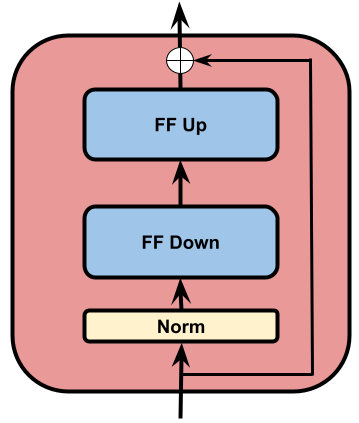
\includegraphics[scale=0.3]{imgs/Adapter_alone.png}
    \caption{Residual Adapter architecture}
    \label{fig:Adapter_architecture}
    \end{center}
    \end{figure*}

    
Adapters were initially introduced in the \ac{NLP} field to efficiently adapt large models, such as Transformers, using a minimal amount of parameters for text classification \cite{houlsby}. As an alternative to full model fine-tuning, Adapter-transfer involves training an extra small number of task-specific parameters while keeping the original model frozen. To this end Adapters are plugged at each Transformer layer level after the \ac{MHA} and \ac{FFN} modules. This setup is often referred to as the \textit{Houlsby} configuration. Subsequently, Pfeiffer \textit{et al.} \cite{pfeiffer} demonstrated that Adapters placed only after the \ac{FFN} modules were sufficient for achieving efficient performances, referred to as the \textit{Pfeiffer} configuration. Typically, Adapters use a bottleneck architecture, consisting of a normalisation layer followed by a projection-down linear layer with a non-linear activation, projecting the input into a $d_{hidden}$ dimension. Subsequently, a projection-up linear layer brings back to dimension $d_{model}$. Finally, a residual connection is applied by summing the input of the Adapter with its output. The overall structure is illustrated in Figure \ref{fig:Adapter_architecture}. Research suggests that the hidden dimension, between the down and up projection, may not always benefit from a bottleneck structure, where $d_{hidden} < d_{model}$, and the optimal design may vary depending on the downstream task \cite{houlsby}. In some tasks, a hidden dimension larger than the model size itself, in other words $d_{hidden} > d_{model}$, has been proven more effective \cite{fan2022draft}.

%Some of the main advantages of Adapters are their parameter efficiency and modularity. This efficiency is particularly interesting when working with large pre-trained models, while modularity is valuable when a large number of tasks need to be trained.
Mathematically, the structure of an Adapter can be expressed as follows:

\begin{equation}
    adapter(x) = x + (W_{up}(f(W_{down}g(x)+b_{down})))+ b_{up})
\end{equation}
Where $W_{down}$ and $W_{up}$ denote the weights of the projection-down and projection-up linear layers with respective dimensions of $\mathbb{R}^{d_{model} \times d_{hidden}}$ and $\mathbb{R}^{d_{hidden} \times d_{model}}$, and $b_{down}$ and $b_{up}$ represent the corresponding biases. The function $f(\cdot)$ is a non-linear activation, while $g(\cdot)$ is a layer normalisation or identity function. Finally, $x$ corresponds to the input given to the Adapter.

In terms of computation, Adapters offer the advantage of faster training, given that they update fewer parameters compared to fully fine-tuning models. Nevertheless, there might be a slight processing delay during inference due to the introduction of extra parameters by the Adapters; however, this difference is generally minimal and can be well-managed \cite{ruckle2020adapterdrop}.

% Adapter ASR
Recently, a rising interest has been observed in Adapter-transfer for \ac{ASR} tasks \cite{cappellazzo2023parameter,chen2023efficient,10095837}, particularly owing to its modular nature, which has proven advantageous in the context of multi-lingual \ac{ASR} \cite{kannan2019large, hou2021exploiting, kulkarni2023adapting}. In these studies, distinct Adapters were trained for each language, contributing to enhanced performance compared to a monolingual model and mitigating certain challenges associated with \ac{TL}, such as overfitting. This modular approach provides a tailored solution, as each Adapter designed for a specific language can effectively capture the diverse acoustic characteristics unique to that language.

Moreover, researchers have explored the use of Adapters in the context of \ac{SSL}. Typically, in \ac{SSL}, larger models are employed to capture a diverse range of information from speech, applicable across a broad spectrum of tasks \cite{thomas2022efficient, fan2022draft}. However, the computational cost and scalability to adapt these models for multiple tasks can be challenging. Notably, once the model is fine-tuned for a specific task, the entire model is fixed for that task, and re-loading and re-training the base model are necessary for transferring to a different task. Therefore, the use of Adapters has proven effective in addressing these challenges by providing a modular and parameter-efficient task-specific adaptation.

%Additionally, the effectiveness of Adapters has been extended by addressing challenges related to low-resource and atypical speech recognition scenarios, as investigated by Tomanek et al. \cite{tomanek2021residual}. This underscores the adaptability and robustness of Adapters, particularly in scenarios where data may be limited or exhibit unconventional characteristics.

Finally, the effectiveness of Adapters has also been demonstrated in addressing challenges related to low-resource and atypical speech recognition scenarios \cite{tomanek2021residual}. This underscores the adaptability and robustness of Adapters, particularly in scenarios where data may be limited or exhibit unconventional characteristics. 
%In such scenarios, similarly to children's speech, there is limited availability of labelled data and atypical speech characteristics. As a result, Adapters provide a valuable solution by efficiently adapting large pre-trained models to these challenging tasks. 

% Adapter children
However, the application of Adapters in the context of children's \ac{ASR} has received limited attention, with only one notable study \cite{fan2022draft}. In this study, the authors introduced a novel approach that involved integrating and training Adapters within \ac{SSL} setting, followed by fine-tuning the entire model, including the Adapter weights,  to enhance the modelling of children's speech. This represents a pioneering effort to leverage Adapters for adapting large-scale models to the unique characteristics of children's speech. Nevertheless, it is crucial to note that in this work, the authors updated the entire model along with the Adapter, compromising the parameter efficiency associated with Adapter-transfer. This highlights the need for a more focused investigation into Adapters as a \ac{PETL} method for children's \ac{ASR}. 

\section{Investigating Adapters for Children's ASR}

\begin{figure*}[t]
    \begin{center}
    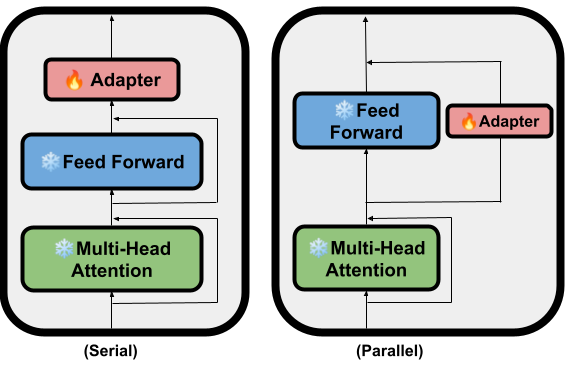
\includegraphics[scale=0.4]{imgs/Adapter_Transformer.png}
    \caption{Transformer block with various residual adapter configurations (Normalisation layers are not shown in this picture for clarity). The fire icon denotes trainable components, whereas the snow icon indicates frozen components.
    }
    \label{fig:transformer_config}
    \end{center}
\end{figure*}
\begin{figure*}[t]
    \begin{center}
    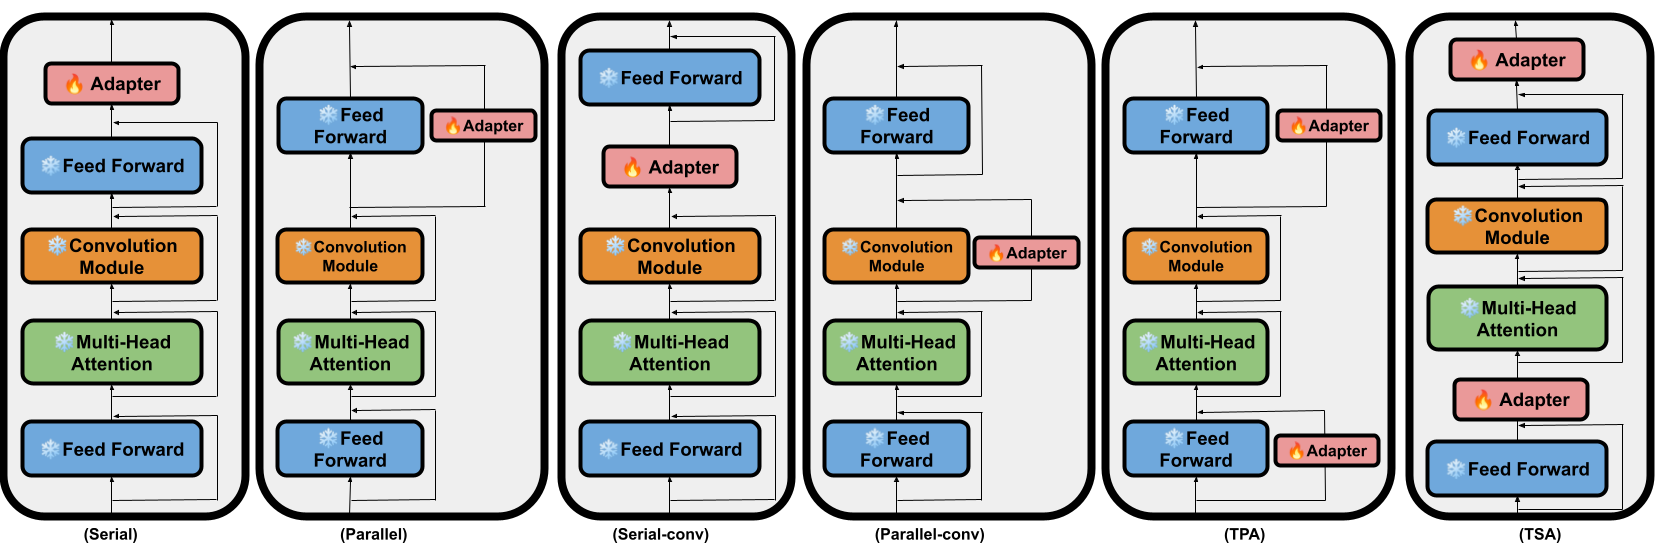
\includegraphics[scale=0.27]{imgs/Adapter_conformer.png}
    \caption{Conformer block with various residual Adapter configurations  (Normalisation layers are not shown in this picture for clarity). The fire icon denotes trainable components, whereas the snow icon indicates frozen components.
    }
    \label{fig:conformer_config}
    \end{center}
\end{figure*}

In this section, we delve into the application of Adapter-transfer as \ac{PETL} for both Transformer and Conformer architectures in the domain of children's \ac{ASR}. Building upon the insights gained from our partial fine-tuning approach in Chapter \ref{chap:4}, we identified \ac{FFN} modules as the most relevant components for fine-tuning in a Transformer-based model. Consequently, we choose to use Adapters for modifying the output of these \ac{FFN} modules. Additionally, given our results that underscored the significance of fine-tuning the Encoder, our primary focus will be on exploring the application of Adapters within the Encoder. For the Transformer architecture, we explore two methods of integrating Adapter modules into the model: \textit{parallel} and \textit{serial} placement with each \ac{FFN} component. These two configurations were used in prior work \cite{he2022towards} and are depicted in Figure \ref{fig:transformer_config}.

In the case of the Conformer architecture, we explore six distinct Adapter configurations, as illustrated in Figure \ref{fig:conformer_config}. The initial two configurations mirror our Transformer investigation, involving both \textit{parallel} and \textit{serial} placements, either after or in parallel with the second \ac{FFN} module \cite{chen2023efficient}. Additionally, we assess a configuration that introduces an Adapter following the convolution module, denoted as the \textit{serial-conv} setup. We evaluate this configuration as it was used in some prior work \cite{10095837}. Notably, although the \ac{FFN} component has been identified as the most crucial for fine-tuning, promising results with our partial fine-tuning have been observed by fine-tuning the convolution modules only. Furthermore, Chen \textit{et al.} \cite{chen2023efficient} introduces two variants of the parallel setup: \textit{parallel-conv} where the Adapter operates in parallel with the convolution module, and the \textit{\ac{TPA}} configuration where two Adapters are placed in parallel with both \ac{FFN} modules in each Conformer layer. 
To comprehensively explore all feasible configurations, we introduce a novel configuration, the \textit{\ac{TSA}}, where two Adapters are sequentially positioned after both \ac{FFN} components in the different Conformer layers. 
This comprehensive exploration of Adapter configurations within both architectures aims to discern the most effective adaptation strategies for children's speech in the context of \ac{ASR}. 


Mathematically, in serial configurations, the Adapter input is provided by the preceding component denoted as $P$, which can be either \ac{FFN} or convolution module, depending on the specific configuration. The output of the Adapter is then determined by the following process:

\begin{equation}
    output =  Adapter(P(x))
\end{equation}

where $x$ represents the input of component $P$.

In parallel configurations, the process varies slightly. In this scenario, the Adapter's input is the same as $P$, and the Adapter's output is combined with the output of component $P$ as follows:

\begin{equation}
    output = x + 0.5 \cdot P(x) + (Adapter(x) - x)
\end{equation}

Furthermore, we consider three distinct configurations where Adapters are integrated into the Decoder. It is important to note that in the Conformer architecture, the Decoder consist of regular Transformer layers. Consequently, we assess both the \textit{Serial} and \textit{Parallel} Adapter setups. Additionally, we examine the combination of the most effective Encoder and Decoder Adapter configurations. To the best of our knowledge, there is no prior research that formally investigates the influence of Adapters within an \ac{ASR} Decoder. 

%Moreover, we consider three distinct configurations where Adapters are placed in the Decoder. It is important to note that in the Conformer architecture, the Decoder is a regular Transformer. Therefore, we evaluate the \textit{Serial} and \textit{Parallel} setups. Subsequently, we investigate the combination of the most effective Encoder Adapter configuration with both Decoder configurations. To the best of our knowledge, there is no prior research that formally investigates the influence of Adapters within an \ac{ASR} Decoder. 

Finally, motivated by the observed strong correlation between children's speech variability and age \cite{TFchildren}, we explore the possibility of training specialised Adapters. However, considering the individual growth speed of each child may not align with a predefined age, using age groups directly may not effectively capture children with similar acoustic characteristics. Additionally, in many children's speech datasets, age information is often not provided. To address this, we propose to partition the dataset into groups of speakers with similar acoustic characteristics based on unsupervised clustering of speaker embeddings.
In practice, we apply a k-means clustering algorithm on the x-vector representation \cite{snyder2018x} of all training utterances. Subsequently, distinct Adapters are trained for each speaker cluster separately. During the testing phase, the closest cluster of the group of speakers is determined for each test utterance, and the corresponding Adapters specific to that group are employed for decoding.
The primary objective of these experiments is to investigate whether Adapters trained on comparable speech characteristics yield improvements over a general Adapter on the entire training set. %Indeed, children's speech is inherently atypical and displays a significant degree of variability, making it imperative to assess the efficacy of existing methods. In prior work, different configurations were employed resulting in a lack of standardised evaluation.

\section{Implementation details}

For all experiments, we used the same pre-trained Transformer and Conformer models described in Section \ref{section:TransformerConformerDetails}. The architecture of each Adapter comprises an initial linear layer projecting to dimension 512 with a \ac{ReLU} activation, followed by another linear layer projecting to dimension 512 with a residual connection from the Adapter input. In the initialisation process for all Adapters, $W_{down}$ was set to all zeros, and $W_{up}$, $b_{down}$, $b_{up}$ were initialised using Xavier initialisation \cite{glorot2010understanding}.

The decision to use a hidden dimension size ($d_{hidden}$) equal to $d_{model}$ instead of employing a bottleneck was influenced by prior research on hidden dimension size. Previous studies consistently demonstrated that larger dimensions tend to result in improved performance scores \cite{chen2023efficient}. All models underwent training of 30 epochs, with a learning rate of $8 \times 10^{-4}$ for training the Adapters and $8 \times 10^{-5}$ for fine-tuning the entire model. In the clustering experiments, we applied the k-means clustering algorithm to the speaker embeddings of each utterance. The speaker embeddings were extracted using a publicly pre-trained ECAPA-TDNN model, trained on adult speech\footnote{https://huggingface.co/speechbrain/spkrec-ecapa-voxceleb}.

For training, we use the My Science Tutor (MyST) Children Speech Corpus, as children dataset. The Myst dataset is the same as it was employed in prior experiments conducted on this dataset within the context of this thesis, as detailed in Table \ref{tab:statistics_myst}. For a more comprehensive understanding of the MyST corpora, additional details are provided in Section \ref{section:children_corpora}.


\section{Results}
\label{sec:results_adapters}

\subsection{Adapter Configurations}
\begin{table}[t]
\begin{center}    
\begin{tabular}{ccc}
\hline
 Method & WER $\downarrow$     & Trained params    \\ \hline \hline
\multicolumn{3}{c}{\textbf{Transformer}} \\ \hline
\multicolumn{1}{l}{\textit{Frozen}} & 25.04\%   & - \\
\multicolumn{1}{l}{\textit{Full fine-tuning}} & 12.99\% & 71.5M \\ \hline
\multicolumn{1}{l}{Serial}  &   12.78\% & 6.3M  \\ 
\multicolumn{1}{l}{Parallel}  &     \textbf{12.62\%} & 6.3M  \\ \hline\hline
\multicolumn{3}{c}{\textbf{Conformer}} \\ \hline
\multicolumn{1}{l}{\textit{Frozen}} & 21.75\%   & - \\ 
\multicolumn{1}{l}{\textit{Full fine-tuning}} & 12.28\% & 109.1M \\ \hline
\multicolumn{1}{l}{Serial}  &   11.76\% & 6.3M  \\ %11.84 
\multicolumn{1}{l}{Serial-Conv} & 11.78\%     & 6.3M  \\
\multicolumn{1}{l}{Parallel}    & 11.72\% & 6.3M  \\ % 11.88 
\multicolumn{1}{l}{Parallel-conv} & 11.79\%      & 6.3M  \\ %\hline
\multicolumn{1}{l}{TPA} & \textbf{11.58\%}     & 12.6M  \\ %11.85
\multicolumn{1}{l}{TSA} & 11.75\%     & 12.6M  \\ \hline %11.72
\multicolumn{1}{l}{Serial (Decoder)} & 18.09\%     & 3.2M  \\ 
\multicolumn{1}{l}{Parallel (Decoder)} &17.76\%     & 3.2M  \\ \hline
%\multicolumn{1}{l}{TPA + Serial (Decoder)} & 00.00(T)\%     & 15.8M  \\
%\multicolumn{1}{l}{TPA + Serial (Decoder)} & 11.68\%     & 15.8M  \\ 
\multicolumn{1}{l}{TPA + Parallel (Decoder)} & \textbf{11.47\%}     & 15.8M  \\ \hline

\end{tabular}
\end{center}
\caption{Results of the different Adapters configurations in both Transformer and Conformer.}
\label{tab:res_config}
\end{table}

In this section, we present a comprehensive evaluation of the different Adapter configurations applied to both Transformer and Conformer models. These results are presented in Table \ref{tab:res_config}. First, we assess the Transformer model when no fine-tuning was applied (\textit{Frozen}), resulting in a \ac{WER} of 25.04\%. Conversely, \textit{Full Fine-Tuning} involved complete fine-tuning of the entire model, working as our baseline system, reducing the \ac{WER} significantly to 12.99\%, with the use of 71.5 million trainable parameters.
Turning to the Adapter setups, we investigate the \textit{Serial} and \textit{Parallel} configurations, both using 6.3 million trainable parameters. The \textit{Parallel} emerged as the best configuration, achieving the lowest \ac{WER} of 12.62\% compared to 12.78\% for the \textit{Serial}. These results underscore the effectiveness of Adapter configurations within the Transformer architecture, as they both perform slightly better than the full-finetuning baseline.

Next, we investigated the Conformer architecture, we once again explored \textit{Frozen} and \textit{Full Fine-Tuning}. The \textit{Frozen} pre-trained model yielded a \ac{WER} of 21.75\%, while the full fine-tuning, in a similar way as the Transformer, led to enhanced performance, with \ac{WER} of 12.28\% using a total of 109.1 million trainable parameters. Within the set of Adapter configurations, \textit{Serial} achieved a \ac{WER} of 11.76\%, while \textit{Parallel} demonstrated slightly better performance with a \ac{WER} of 11.72\%. These results confirm that \textit{Parallel} Adapters were more effective in improving \ac{WER} in both Transformer and Conformer models. When Adapters are placed after the convolution layer, with the \textit{Serial-conv} and \textit{Parallel-conv} configuration, both slightly under-perform compared to Adapters placed after the second \ac{FFN} component with respective scores of 11.78\% and 11.79\%. Finally, we evaluated the \textit{\ac{TPA}}and \textit{\ac{TSA}} configurations. The \textit{\ac{TPA}} configuration emerged as the most promising, with a remarkable \ac{WER} of 11.58\% using 12.6 million trainable parameters, while \textit{\ac{TSA}} achieved a \ac{WER} of 11.75\%, which is slightly under-performing compared to the \textit{\ac{TPA}} configuration.

In addition, we evaluated the use of Adapters in the Decoder. As the Decoder of the Conformer architecture is a regular Transformer, we only evaluate the \textit{Serial} and \textit{Parallel} setup, which respectively reached 18.09\%  and 17.76\% \ac{WER} with 3.2 million parameters. These results showed that Adapters are more relevant when plugged into the Encoder which is in line with findings from Chapter \ref{chap:4}. Finally, combining \textit{\ac{TPA}} in the Encoder layers with \textit{Parallel} Adapters in the Decoder outperforms Adapters in the Encoder only, with 11.47\% \ac{WER}. Consequently, this configuration stands as the most effective configuration for our children's speech dataset. 

%statistical tests
We performed statistical tests (Matched Pairs Sentence-Segment Word Error) across all Adapter setups in comparison to the full fine-tuning configuration using SCTK, the NIST Scoring Toolkit \footnote{https://github.com/usnistgov/SCTK/tree/master}. 
The results reveal that, in all scenarios, the \textit{p}-value is less than or equal to 0.001. This observation denotes statistical significance, indicating evidence against the null hypothesis. 

These results collectively illustrate the versatility and effectiveness of different Adapter configurations within the Transformer and  Conformer model for the children's \ac{ASR} task. \textit{\ac{TPA}} Adapters in the Encoder combined with \textit{Parallel} Adapters in the Decoder showcased outstanding performance, highlighting their potential as a fine-tuning replacement in large model children \ac{ASR} scenarios.

\subsection{Effect of the Adapters hidden dimension}
\label{sec:hidden_size_adapter}
\begin{figure}
    \begin{center}
    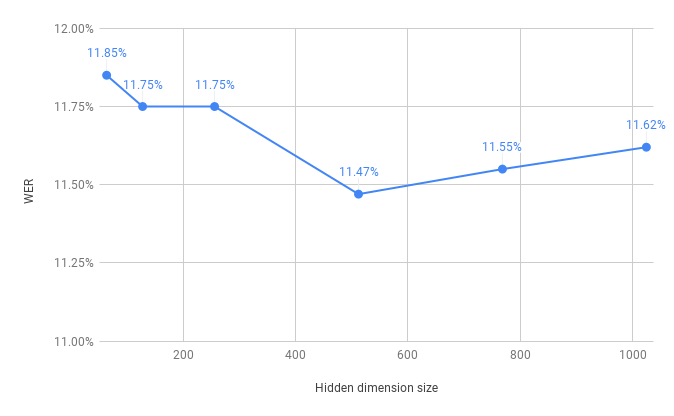
\includegraphics[scale=0.5]{imgs/HiddenDimEXP.png}
    \caption{Experimental Adapter transfer using different hidden dimension sizes within the Conformer architecture.}
    \label{fig:HiddenDim}    
\end{center}
    
\end{figure}

In this section, our objective is to assess the influence of different hidden dimension values for the Adapter ($d_{hidden}$) on the model's performance. In our previous experiments, we maintained a fixed hidden dimension, where $d_{model} = d_{hidden} = 512$. Now, we aim to explore various hidden dimension values within the Conformer architecture, focusing on the \textit{\ac{TPA}} in the Encoder-only configuration. This investigation aims to assess how variations in the hidden dimension may impact the performance of the Adapter transfer, offering valuable insights into the parameter tuning process for Adapter modules.

In Figure \ref{fig:HiddenDim}, the relative \ac{WER} delta compared to the full model fine-tuning performances of the Adapter transfer are presented in relation to the hidden dimension size ($d_{hidden}$), and therefore the relative amount of parameters compared to the entire model. Notably, a trade-off is observed, emphasising the importance of choosing an optimal hidden dimension size. Configurations with dimensions that are either too small or too large result in a degradation of overall performance. The best-performing configuration aligns with the choices made in all previous experiments, with $d_{hidden} = d_{model} = 512$. We hypothesise that the parallel Adapter functions as an extension of the key-value memory of the \ac{FFN}. Opting for an extremely large hidden dimension makes training more complex due to a large number of parameters, while an excessively small size drastically limits the potential information learned from the Adapters. 

\subsection{Unsupervised clustering for grouped-speaker Adapters}
\label{sec:clustering_emb}
\begin{table}[t]
    \begin{center}    
    \begin{tabular}{cc}
    \hline
      \# of clusters & Average WER $\downarrow$    \\ \hline
    \multicolumn{1}{c}{1} & 11.58\%  \\% OR 11.70%  If we consider 40 epochs instead of 30 here
    \multicolumn{1}{c}{2} & \textbf{11.50\%}  \\
    \multicolumn{1}{c}{3} & 11.57\%  \\
    \multicolumn{1}{c}{4} & 11.51\%  \\ \hline 
    \end{tabular}
    \end{center}
    \caption{Results of the unsupervised clustered Adapters approach.}
    \label{tab:res_clusters}
    \end{table}


In this section, we present the outcomes of our clustering approach summarised in Table \ref{tab:res_clusters}. The investigation focuses on the influence of varying the number of clusters on the \ac{ASR} scores, ranging from 1 to 4 clusters, using the \textit{\ac{TPA}} configuration in an Encoder-only setup within the Conformer model.

Initially, when the data remained unclustered, corresponding to one cluster, the \ac{ASR} system exhibited a \ac{WER} of 11.58\%. Notably, the two-cluster configuration outperformed the other setups, achieving superior performance with a \ac{WER} of 11.50\%. This result suggests that partitioning the data into two distinct clusters allows the different Adapters to more effectively capture underlying patterns intricately linked to their respective clusters, consequently enhancing the recognition scores.

Furthermore, we explored the impact of increasing the number of clusters to three and four, revealing only marginal differences in performance. Specifically, the three-cluster configuration yielded a \ac{WER} of 11.57\%, and the four-cluster configuration resulted in a \ac{WER} of 11.51\%. These findings underscore the role of data clustering in children's \ac{ASR} systems by grouping shared speaker characteristics into different clusters.


In summary, our investigation emphasises the role of data clustering in the context of children's \ac{ASR} systems. Specifically, for the Myst dataset, optimal performance was attained with a two-cluster configuration, suggesting that this approach facilitates the effective capturing of cluster-specific patterns by the Adapters. The marginal performance differences observed with three and four clusters suggest a potential saturation point, indicating that further partitioning may yield diminishing returns in terms of \ac{ASR} performance improvement for this specific dataset.

It is noteworthy that, in this experiment, the amount of available training data for Adapters varies due to the clustering process. A more comprehensive exploration of the impact of training hours on Adapters will be presented in Section \ref{sec:hours_PETL}. This forthcoming analysis will offer a detailed understanding of how different training amount of data influence the performance of Adapters in diverse conditions, shedding light on their adaptability and effectiveness across various scenarios.

Additionally, considering the relatively narrow age range of the Myst corpus, encompassing children from the third to fifth grade, future work could explore the applicability of this approach on children datasets with a more extensive age range. This extension would contribute valuable insights into the generalisation and robustness of the clustering-based Adapter approach across diverse age groups within the realm of children's \ac{ASR}.

    
\section{Summary and discussion}
% Summary
In this chapter, we investigated the viability of Adapter-transfer in the context of children's \ac{ASR}. Addressing the research question, \textit{Does parameter efficient transfer improve children \ac{ASR} compared to full model fine-tuning?} our investigation yielded an affirmative response. Our study showcased the effectiveness of adapting the model using Adapter modules, resulting in improved \ac{WER} performances compared to full-model fine-tuning. Notably, this was achieved while utilising only approximately 10\% of the parameters required in the traditional transfer learning of the entire model, underscoring the parameter efficiency of Adapter-transfer.
 
Among the various configurations explored in this chapter, the ``parallel" Adapter and its extension, the ``\ac{TPA})" emerged as the most effective choices for the Transformer and Conformer architectures, respectively. The ``parallel" Adapter, in particular, demonstrated its efficacy as it extends the key-value memory that represents the \ac{FFN} modules \cite{geva2020transformer}, showcasing its potential to capture essential information specific to children in a more parameter-efficient manner.

Building on these findings, we proposed the integration of unsupervised clustering on the speaker embeddings extracted from different utterances into the Adapter-transfer procedure. This strategic clustering aimed to facilitate the training of specific Adapters for each cluster, offering a more personalised adaptation without relying on detailed metadata about the speaker, such as their age. Our results illustrated that leveraging these clusters could further enhance overall performances, opening avenues for the application of Adapters for better personalised \ac{ASR} systems.


% Discussion
% Mention that this opens the way for other uses, such as reducing the domain mismatch
The successful implementation of Adapter transfer in the domain of children's speech presents promising opportunities for advancing children's \ac{ASR}. Our findings indicate that Adapters serve as effective tools for bridging the gap between a source and a target domain while retaining the valuable knowledge encapsulated in pre-trained models. This promising outcome lays the foundation for further exploration. In the upcoming chapter, we will extend our research by investigating the application of Adapters in the domain of \ac{TTS} data augmentation. This extension aims to leverage the capabilities of Adapters to reduce the disparity between real and synthetic children's speech.

% Also mention that we will investigate other PETL approaches
Moreover, in addition to the Adapter module introduced in this chapter, it is noteworthy to mention that various \ac{PETL} alternatives exist in the literature, demonstrating their effectiveness in tasks beyond children's \ac{ASR}, such as \ac{NLP} tasks demonstrating in some scenario better accuracy and parameter efficiency. Therefore, in the next chapter, we will extend our exploration of \ac{PETL} modules, evaluating their applicability and performance in the specific context of children's \ac{ASR}. Additionally, we will delve into the development of new \ac{PETL} approaches, aiming to strike a better balance between parameter efficiency and accuracy. 


